\chapter{System Model}
\label{chap:model}
% system flow diagram
% UE generation method
% satellite beams to cells selection
% satellite orbit pattern

\section{LEO Satellite Communication System}
This chapter introduces the LEO satellite communication system, as illustrated in Figure~\ref{fig_system}. There are $N$ satellites, denoted as $\mathcal{N} = \{n \mid n = 1, 2, \ldots, N\}$, and each satellite has $M$ beams, denoted as $\mathcal{M} = \{m \mid m = 1, 2, \ldots, M\}$. The coverage area consists of $K$ ground cells, denoted as $\mathcal{K} = \{k \mid k = 1, 2, \ldots, K\}$. There are $U$ user equipments (UEs) in the coverage area, denoted as $\mathcal{U} = \{u \mid u = 1, 2, \ldots, U\}$. A hexagonal grid of cells and the quasi-earth-fixed cell scheme are considered. For each satellite, 

\begin{figure}[h!]
    \centering
    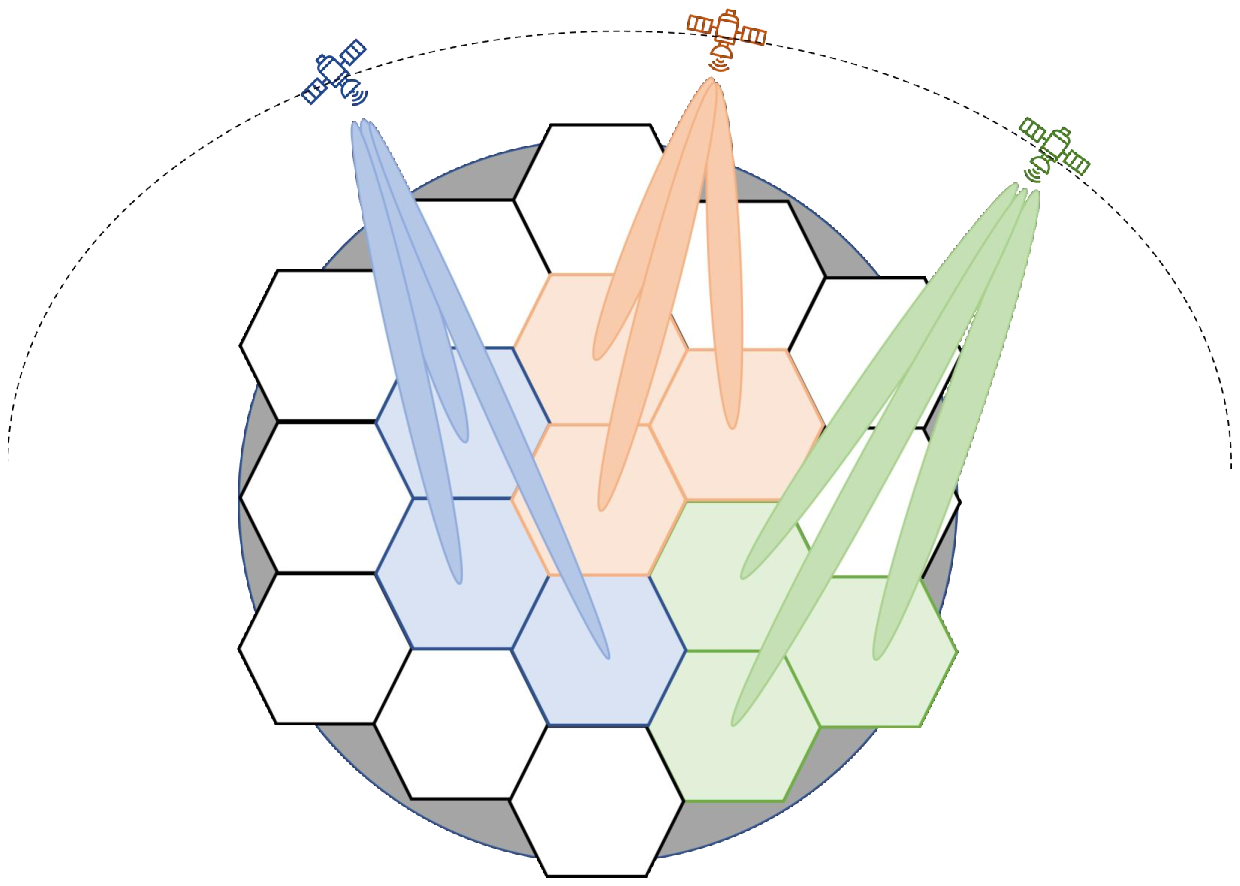
\includegraphics[width=0.8\textwidth]{figure/system overview.pdf}
    \caption{Illustration of satellite beams and cells.}
    \label{fig_system}
\end{figure}

\section{Channel Model}

\subsection{Free Space Path Loss}
In the LEO satellite system, the free space path loss from satellite $n$ to cell $k$ is expressed as follows~\cite{Satellite-Multi-Beam}:
\begin{equation}
    L_{n,k} = \left(\frac{\lambda}{4\pi d_{n,k}}\right)^2
\end{equation}
where $\lambda$ is the wavelength, and $d_{n,k}$ is the distance between the $n$-th satellite and the center of the $k$-th cell.

\subsection{Shadowed-Rician Fading Channel}
The shadowed-Rician fading model is suitable for satellite communication systems because it accurately reflects the physical propagation environment, capturing both the presence of a strong line-of-sight (LoS) signal and the effects of shadowing from obstacles~\cite{channel-model}. Let $h_{n,k}$ denote the channel gain between the $n$-th satellite and the $k$-th cell. The cumulative distribution function (CDF) of the channel gain is:
\begin{equation}
    F_{h_{n,k}}(x) = K \sum_{n=0}^{\infty} \frac{(m)_n \, \delta^n \, (2b)^{1+n}}{(n!)^2} \, \gamma\left(1+n, \frac{x}{2b}\right)
\end{equation}
where $K = \left(\frac{2bm}{2bm+\Omega}\right)^m/2b$, $\delta = \Omega/(2bm+\Omega)/2b$, $\Omega$ is the average power of the LoS component, $2b$ is the average power of the multipath component except the LoS component, and $m$ is the Nakagami parameter.

\subsection{Antenna Radiation Pattern}
We introduce the antenna radiation pattern in~\cite{Energy-Efficient}:
\begin{equation}
    G(\theta_{n,m,u}) = G_{max} \left[ \frac{J_1\left(\mu(\theta_{n,m,u})\right)}{2\mu(\theta_{n,m,u})}
    + 36 \frac{J_3\left(\mu(\theta_{n,m,u})\right)}{\mu(\theta_{n,m,u})^3} \right]^2
\end{equation}
where $\theta_{n,m,u}$ is the boresight angle between the user position and the beam center with respect to the satellite, $G_{max}$ is the maximum antenna gain, $\mu(\theta)$ is defined as $2.07123 \cdot \sin(\theta)/\sin(\theta_{3dB})$, $\theta_{3dB}$ is the 3 dB half-power beamwidth angle of the antenna, and $J_1(\cdot)$, $J_3(\cdot)$ are the Bessel functions of the first kind of orders 1 and 3, respectively.

With the transmitted power $P_{n,m}$ from the $m$-th beam of the $n$-th satellite, the received power at the $u$-th user, $\hat{P}_{n,m,u}$, is given by:
\begin{equation}
    \hat{P}_{n,m,u} = P_{n,m} \cdot L_{n,k} \cdot h_{n,k} \cdot G(\theta_{n,m,u})
\end{equation}
where $k$ is the cell where user $u$ is located.

\section{Synchronization Signal Block Model}
This section describes the SSB periodicity settings based on 3GPP protocol and their impact on system operation. According to 3GPP protocol~\cite{38331}, the supported synchronization signal block (SSB) periodicity values are $\{20, 40, 80, 160\}$ milliseconds. The SSB periodicity of each cell is defined as:
\begin{equation}
    T^{SSB}_{k} \in \{20, 40, 80, 160\}, \quad \forall k \in \mathcal{K}
\end{equation}

The duration of each time slot is set to 160 ms. To simplify computational complexity, both the positions of satellites and UEs are assumed fixed within each time slot. The SSB periodicity specification for each cell remains unchanged throughout the slot.

Let $\Delta_{n,m}[t]$ denote the set of cells served by the $m$-th beam of the $n$-th satellite at time slot $t$. Since the time duration of each slot is 160 ms and the SSB periodicity is 20, 40, 80, or 160 ms, the number of elements in $\Delta_{n,m}[t]$ must be 1, 2, 4, or 8, as shown in Figure~\ref{delta}.

\begin{figure}[h!]
    \centering
    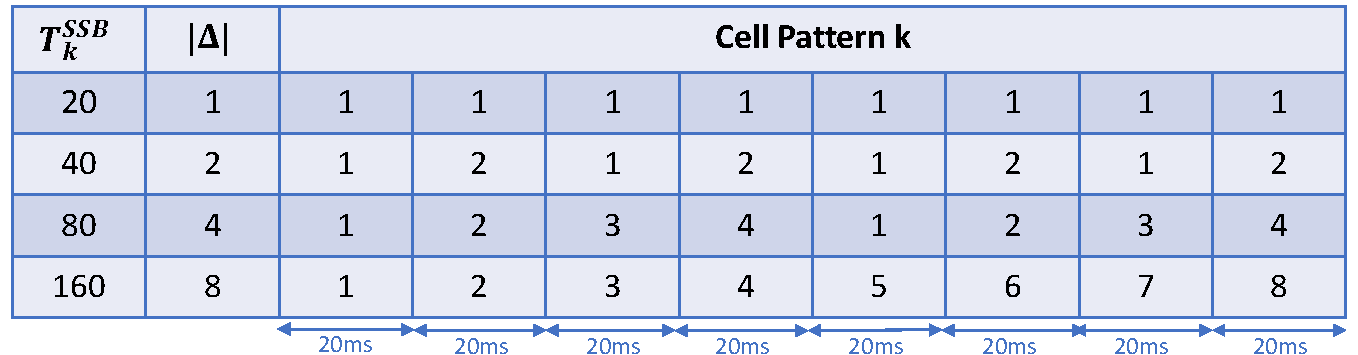
\includegraphics[width=0.8\textwidth]{figure/delta pattern.pdf}
    \caption{Illustration of SSB periodicity and cell patterns for different periodicity settings.}
    \label{delta}
\end{figure}

\section{UE Random Access Delay}
The random access delay $T_u$ for the $u$-th UE is defined as the time duration between the start of SSB measurement and the successful reception of SSB, as shown in Figure~\ref{RAD}. $T_u$ can be decomposed into two parts: $T_u^i$ (initial waiting time) and $T_u^l$ (additional delay due to failed attempts). $T_u^i$ is the time from the start of SSB measurement to the arrival of the first SSB, and $T_u^l$ is the time from the first SSB arrival to the successful SSB reception.

Since the UE can start SSB measurement at any time, $T_u^i$ is a uniformly distributed random variable $U(0, T_{k_u}^{SSB})$. $T_u^l$ is a multiple of $T_{k_u}^{SSB}$, depending on the number of failures $Q_u$. If the received SSB power $\hat{P}_{n, m, u}$ is less than the threshold $P_{th}$, the UE fails to measure SSB. The probability that the received SSB power is less than $P_{th}$ is denoted as $P_u^0$. The mathematical formulation is as follows:
\begin{equation}
    T_u = T_u^i + T_u^l
\end{equation}
\begin{equation}
    F_{T_u^i}(t) =
    \begin{cases}
        \frac{t}{T_{k_u}^{SSB}}, & 0 \leq t < T_{k_u}^{SSB} \\
        1, & t \geq T_{k_u}^{SSB} \\
        0, & \text{otherwise}
    \end{cases}
\end{equation}
\begin{equation}
    T_u^l = Q_u \cdot T_{k_u}^{SSB}
\end{equation}
\begin{equation}
    \Pr\left[Q_u = n\right] = (1 - P_u^0) (P_u^0)^n
\end{equation}
where $k_u$ is the cell where the $u$-th UE is located.

\begin{figure}[h!]
    \centering
    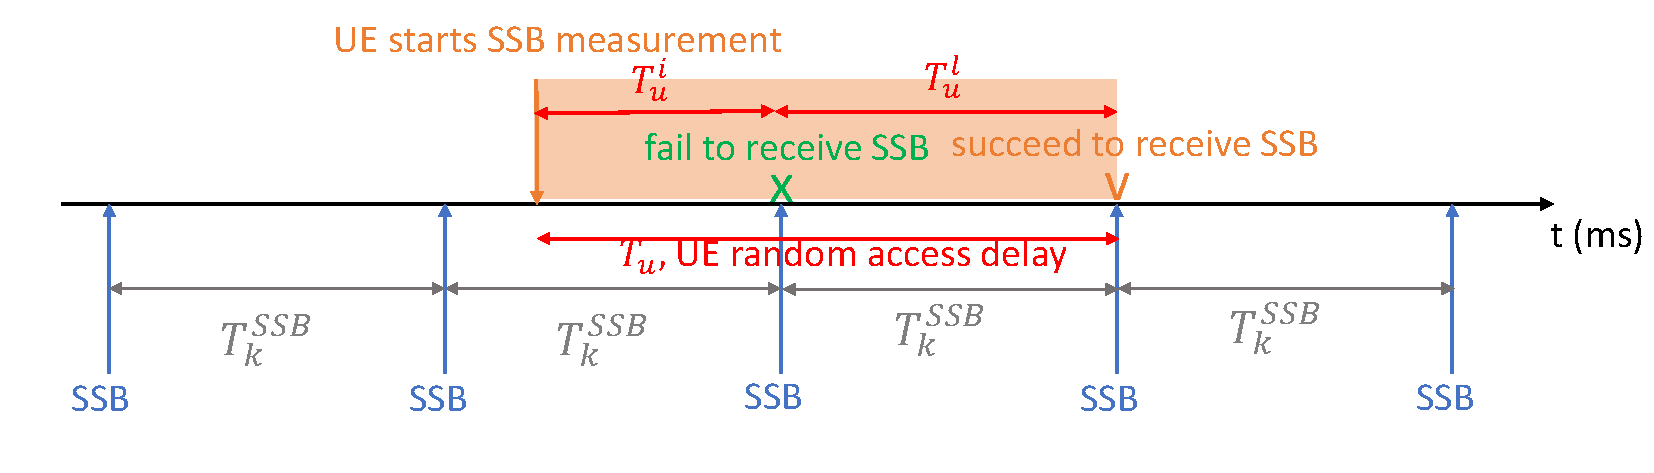
\includegraphics[width=1\textwidth]{figure/random access delay.pdf}
    \caption{Illustration of UE random access delay. $T_u$ is decomposed into $T_u^i$ (initial waiting time) and $T_u^l$ (additional delay due to failed attempts).}
    \label{RAD}
\end{figure}

\section{Problem Formulation}
This section formulates the optimization problem based on recent 3GPP standardization discussions. In the 3GPP RAN1 \#116 meeting~\cite{ran1-116}, further specifications for the LEO satellite communication scenario were defined. The main challenge is to provide random access to a large number of cells with limited satellite power. Extending the SSB periodicity for some cells reduces satellite power consumption but increases UE random access delay. The transmitted SSB power also affects the success probability of the random access procedure. The trade-off among power allocation, SSB periodicity, and UE random access delay is modeled as follows:
\begin{equation}
\begin{aligned}
    & \underset{\Delta, P_{n, m}}{\text{min}} \sum_{u \in \mathcal{U}} T_u \\
    & \text{subject to} \\
    & \quad \sum_{m} P_{n,m}[t] \leq P_s, \quad \forall n \in \mathcal{N} \\
    & \quad \Delta_{n, m}[t] \in \{0, 1, 2, 4, 8\}, \quad \forall n \in \mathcal{N}, m \in \mathcal{M} \\
    & \quad \Delta_{n, m}[t] \cap \Delta_{n', m'}[t] = \emptyset, \quad \forall n, n' \in \mathcal{N}, m, m' \in \mathcal{M}, (n, m) \neq (n', m')
\end{aligned}
\end{equation}
where $P_s$ is the maximum transmitted power for each satellite.

\section*{List of Symbols}
\begin{tabular}{ll}
$N$ & Number of satellites \\
$M$ & Number of beams per satellite \\
$K$ & Number of cells on the ground \\
$U$ & Number of user equipments (UEs) \\
$L_{n,k}$ & Free space path loss from satellite $n$ to cell $k$ \\
$h_{n,k}$ & Channel gain between satellite $n$ and cell $k$ \\
$G(\theta_{n,m,u})$ & Antenna gain for user $u$ \\
$T^{SSB}_k$ & SSB periodicity of cell $k$ \\
$T_u$ & Random access delay of UE $u$ \\
$P_{n,m}$ & Transmitted power of satellite $n$'s $m$-th beam \\
$P_s$ & Maximum transmitted power for each satellite \\
$P_{th}$ & SSB reception threshold \\
$Q_u$ & Number of failed SSB attempts for UE $u$ \\
\end{tabular}
